\documentclass[12pt]{article}

\usepackage[margin=0.75in]{geometry}
\usepackage{graphicx}
\usepackage{float}

\newcommand{\graphwidth}{0.5\linewidth}

%\graphicspath{ {./res/image/}}


\title{ {\Huge Dual Rail Power Supply } \\
    ECE 302 Lab \#1 \\ LAD D11 / Bench \#9}
\author{
    Lyndon Sanche\\
    \texttt{lsanche@ualberta.ca}
    \and
    David Lenfesty\\
    \texttt{lenfesty@ualberta.ca}
}

\begin{document}
\pagenumbering{roman}

\maketitle


\section{Abstract}

Low-noise, low power split rail power supplies are a staple of the audio industry.
In order to generate the required audio waveforms for applications such as headphone or
low-power amplifiers, a negative and a positive voltage rail is necessary.

In this lab, a $\pm10 V$ split rail power supply was implemented, 
where the output ripple was designed to be less than $ 0.5 \% $ of the
regulated voltage. This supply operated using mains $115 V_RMS$, $60Hz $ power, with
a step down transformer leading to a diode rectifier. This rectifier supplied DC power to
positive and negative rails, each using a capacitor as a low-pass filter and implementing
a regulator output. The positive rail used an off the shelf 78L10AC linear regulator,
while the negative rail used a Zener diode-based regulator circuit.

\pagenumbering{arabic}

\section{Objectives}

The objective of this lab is to design a split-rail power supply capable of supplying
$\pm 10V$ at 25mA, with a voltage error of less than 5\% and less than 0.5\% ripple.

This power supply will be used later in this lab to provide power for the audio amplifier
we will design.

\section{Design}

In order to simplify the design process, the power supply design was split into three
stages, rectification, filtering, and regulation. By splitting up the design into these
parts, it was simpler to test and easier to diagnose issues.
The purpose of this power supply is to take a $60\,Hz$, $120 V_{RMS}$ signal, and convert it to a $\pm10 V$ DC signal. The circuit is divided into
several stages for easier understanding, design, and testing. These stages include a transformer stage, rectifier stage, filter stage, and regulator stage. The combination 
of these stages allow us to convert a $120 V_{RMS}$ signal from a standard wall outlet, and convert it into two rails, one supplying roughly $10 V$ and one supplying $-10 V$. 
The supply is designed to have a minimal amount of ripple so the current going into the load does not fluctuate.

By simulating the circuit prior to building it, we were able to experiment wth different
component values and the effects of removing certain key components, which gave a better
understanding of how the circuit worked.

\subsection{Transformer}
The transformer stage is used to step down the $120 V_{RMS}$ voltage down to a voltage that will be manageable by the rectifier, filter, and regulator stages.

\subsection{Rectifier}
The rectifier stage is the first part of converting our signal to positive and negative rails. We have chosen to use a full-bridge rectifier design as it converts all parts of the voltage signal 
to be positive or negative, depending on the rail, and produces a more uniform and efficient output compared to half-wave or full-wave rectifiers. We have chosen the bridge rectifier instead of a rectifier design such as a half wave rectifier, as it doesn't cut out 
the negative parts of our wave, flipping them instead so we have more consistent voltage in our supply. We hook up the positive and negative rails to the same rectifier to produce a 
positive and negative rectified signal.

\subsection{Filter}
For the filter stage, we chose to use a shunt capacitor filter. The rectified AC signal that comes from the bridge rectifier is not appropriate to power electronic devices, so 
we use the capacitor filter to smooth out the output. We have chosen an appropriate capacitance to filter out a large amount of the AC components of our signal, leaving us a 
signal that stays around 10V with a manageable mount of ripple.

The largest size capacitor available in the lab kit was the one that was eventually chosen,
at $100 \mu F$, it provided plenty of filtering and smoothed out the rectifier waveform
well enough to limit ripple significantly.

\subsection{Regulator}
The regulator stage is different on the positive and negative rail. For the positive rail, we use a voltage regulator to remove the ripple on the signal, making it a 
near constant $\pm10 V$ DC signal. We find that the voltage regulator is very effective at removing ripple from our signal.

\subsection{Zener Regulator}
For the negative rail, we make use of a zener diode to regulate our voltage. Zener diodes are effective at regulating voltage when paired with the right ballast resistor. Even 
with the right ballast resistance, we were having some trouble removing the ripple from our signal, we put a capacitor in parallel with our load to regulate the voltage further. 
The result of this design is an effective voltage regulator, however, it is not as effective as a stand-alone voltage regulator.

For the filter stage, we chose to use a shunt capacitor filter. The rectified AC signal that comes from the bridge rectifier is not appropriate to power electronic devices, so we use the capacitor filter to smooth out the output. We have chosen 
an appropriate size of capacitor to filter out a large amount of the AC components of our signal, leaving us a signal that stays around 10V with a manageable mount of ripple.

The regulator stage is different on the positive and negative rail. For the positive rail, we use a voltage regulator to remove the ripple on the signal, making it a near constant 10V dc signal. We find that the voltage regulator is very effective at removing 
ripple from our signal.

For the negative rail, we make use of a zener diode to regulate our voltage. Zener diodes are effective at regulating voltage when paired with the right ballast resistor. Even with the right ballast resistance, we were having some trouble removing the ripple from our signal, 
we put a capacitor in parallel with our load to regulate the voltage further. The result of this design is an effective voltage regulator, however, it is not as effective as a stand-alone voltage regulator.

\subsection{Future Use}
After all these stages the power supply will output 10 volts on a positive and negative rail. These two rails will be useful when designing an audio amplifier, as we'll need control over the 
positive and negative voltages of audio signals.


The final circuit schematic can be found in appendix (\ref{app:circuit}).

\section{Simulation}

\section{Results}


\section{Discussion}


The zener diode performs worse than the IC-based linear regulator. The linear regulator consumes less quiescent current to do the regulation,
and also has better ripple-rejection than the zener regulator.

While the zener diode required a small-sized ballast resistor and an extra capacitor on the output to reduce ripple,
the IC regulator did this without any extra components, and was simpler to design around, requiring less calculations
and tweaking.

This design used a low-pass filter (LPF) because a purely DC signal was wanted, with no
AC components, as those would manifest as noise on the final output of the amplifier.

Additional filtering was needed for the zener regulator to keep the ripple down. This was adjusted
simply by testing different capacitances.

This power supply design was quite inefficient, having to drop around $10V$ to provide the correct
output. This could easily be improved by changing the transformer to one with twice the windings on
one side to drop the voltage even more before regulation and filtering.

There is a difference between the calculations, the simulations, and the measurements, because the
calculations were simplified formulas, the simulations assumed perfect components, and the
measurements used components that had parasitics and uncertainties.

The major difficulty we faced was with the ripple on the zener output. We did a 
calculation over again in the lab and didn't reference our notes, so we got stuck
on a higher value ballast resistor than necessary. This could simply have been fixed by referencing
our notes properly.

\section{Conclusion}
Designing a power supply in lab allowed us to test different configurations to create a functional source of power for future projects. 
Using different regulators for the two rails allows us to test and compare the two designs side by side. We can see in our testing that a voltage regulator IC is much more effective 
in voltage regulation than a zener diode.

The power supply designed has shown to be effective at providing a reliable DC signal with minimal ripple, showing that the combination of rectifier, filter, and regulator is effective 
at converting an AC signal to a DC signal. Slight changes to certain parts of the design could easily make the power supply work for different use cases, such as changing the rail voltages.

For this lab, a series of requirements was laid out for designing a power supply for an audio
amplifier. These requirements were taken and turned into a functional circuit that met
all of the requirements. In this lab, we were able to effectively use diodes to create
a functioning full-bridge rectifier, turning AC current into DC current, and then filter
and regulate this signal using a capacitors, an off-the-shelf voltage regulator IC, and
a zener diode.

\newpage

\begin{appendix}

\section{Simulation Circuit}
\label{app:simulation}

\begin{figure}[H]
    \centering
    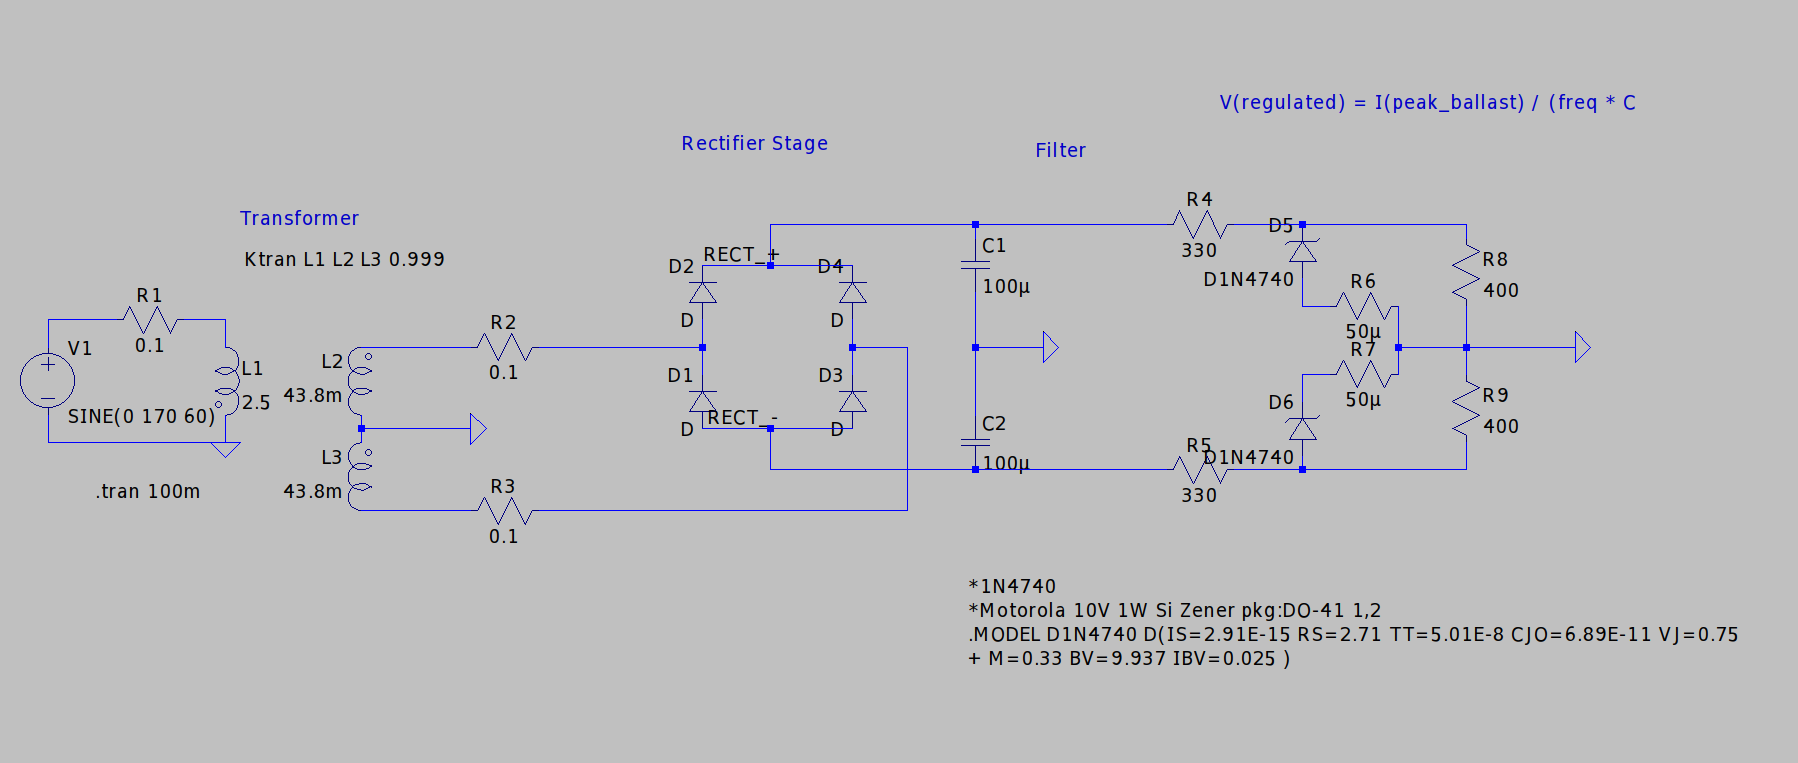
\includegraphics[width=\linewidth]{./SPICE/circuit.png}
    \caption{Complete simulated circuit.}
    \label{fig:simulated_circuit}
\end{figure}

\section{Final Circuit}
\label{app:circuit}

\begin{figure}[H]
    \centering
    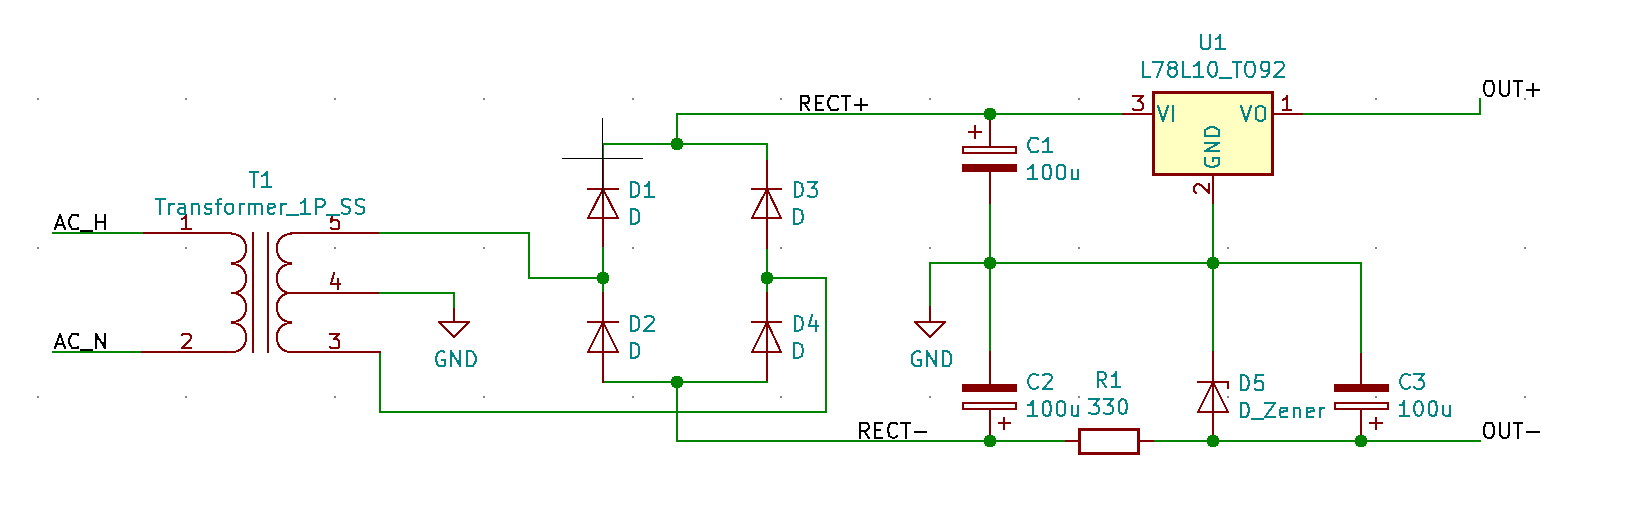
\includegraphics[width=\linewidth]{./res/image/circuit.png}
    \caption{Final circuit.}
    \label{fig:final_circuit}
\end{figure}

\newpage

\section{Rectifier Waveforms}

\subsection{Simulated}

\begin{figure}[H]
    \centering
    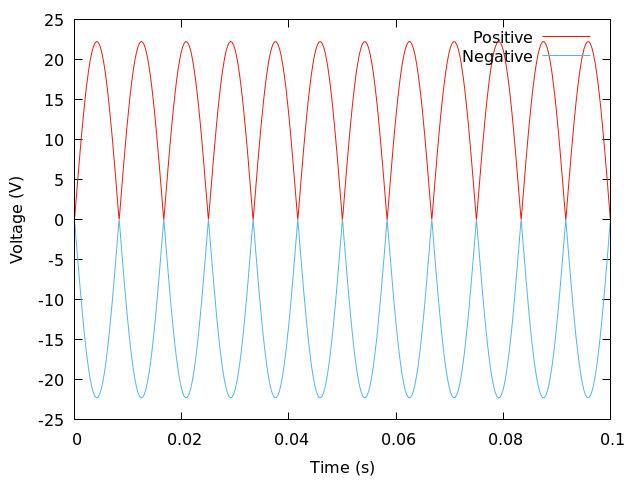
\includegraphics[width=\graphwidth]{./res/image/sim-rectifier-unfiltered.png}
    \caption{Simulated rectifier outputs, both positive and negative.}
    \label{sim:rectifier_unfiltered}
\end{figure}

\subsection{Measured}

\begin{figure}[H]
    \centering
    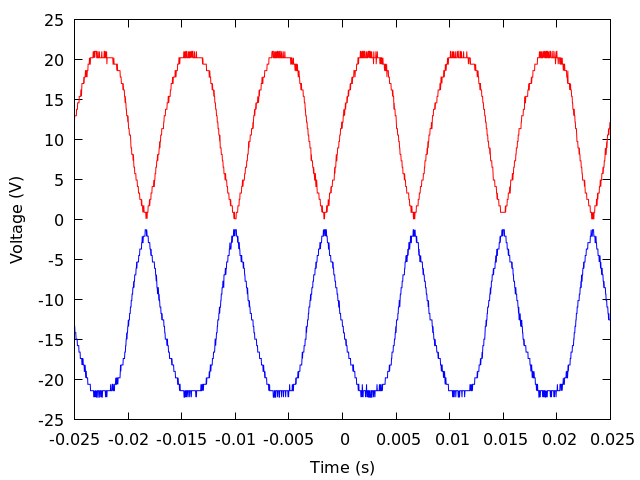
\includegraphics[width=\graphwidth]{./res/image/rectifier-output.png}
    \caption{Actual rectifier outputs.}
    \label{fig:rectifier_unfiltered}
\end{figure}

\section{Filter Waveforms}

\subsection{Simulated}

\begin{figure}[H]
    \centering
    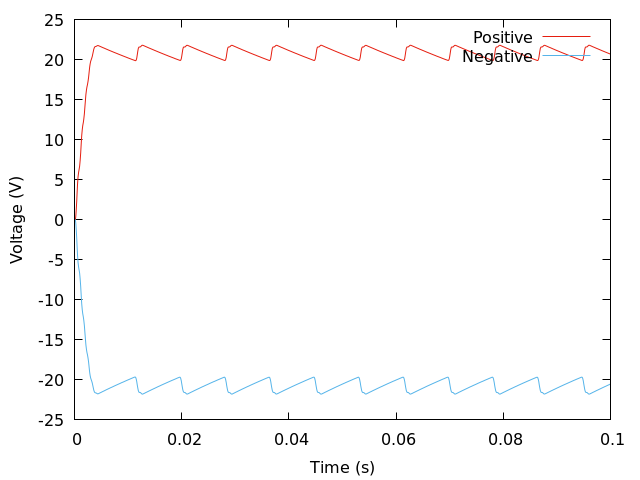
\includegraphics[width=\graphwidth]{./res/image/sim-filtered.png}
    \caption{Simulated filter outputs.}
    \label{sim:filtered}
\end{figure}

\subsection{Measured}

\begin{figure}[H]
    \centering
    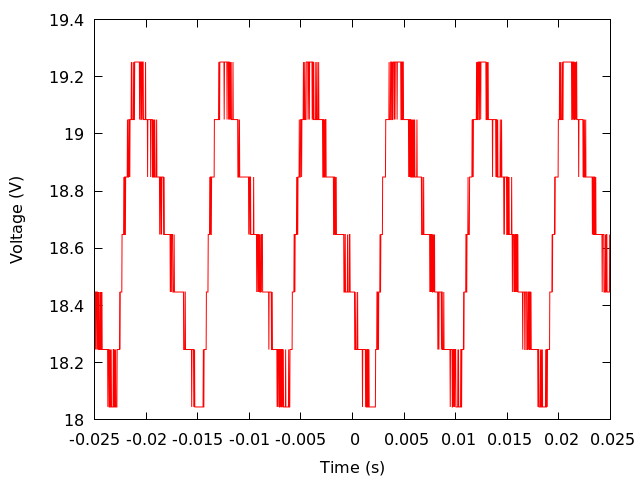
\includegraphics[width=\graphwidth]{./res/image/rectifier-withload.png}
    \caption{Measured filter output.}
    \label{fig:filtered}
\end{figure}

\section{Regulator Waveforms}

\subsection{Positive Regulator}

\subsubsection{Measured}

\begin{figure}[H]
    \centering
    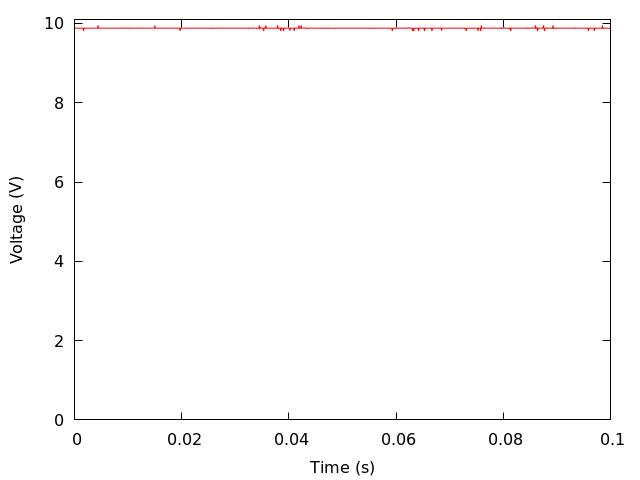
\includegraphics[width=\graphwidth]{./res/image/pos-fullload.png}
    \caption{Measured full load positive rectifier output.}
    \label{fig:pos_fullload}
\end{figure}

\begin{figure}[H]
    \centering
    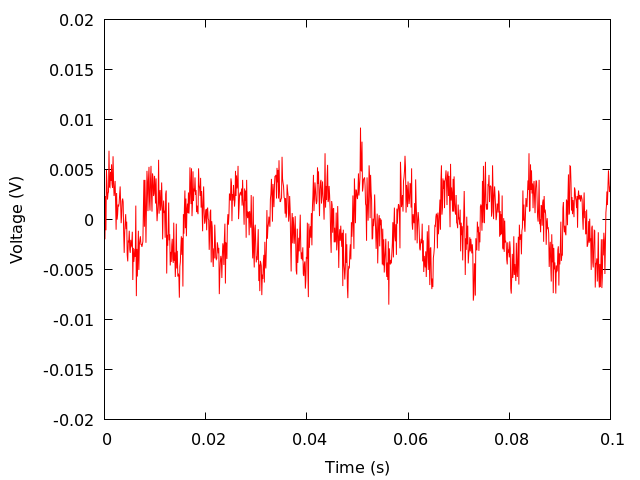
\includegraphics[width=\graphwidth]{./res/image/pos-fullload-ripple.png}
    \caption{Measured full load positive rectifier ripple.}
    \label{fig:pos_fullload_ripple}
\end{figure}

\begin{figure}[H]
    \centering
    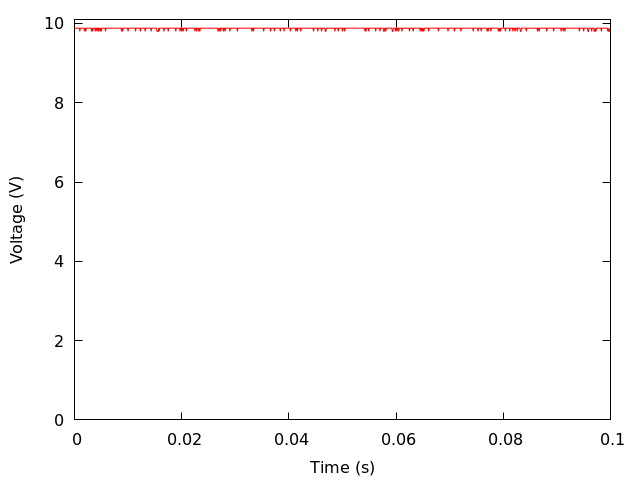
\includegraphics[width=\graphwidth]{./res/image/pos-noload.png}
    \caption{Measured no load positive rectifier output.}
    \label{fig:pos_noload}
\end{figure}

\begin{figure}[H]
    \centering
    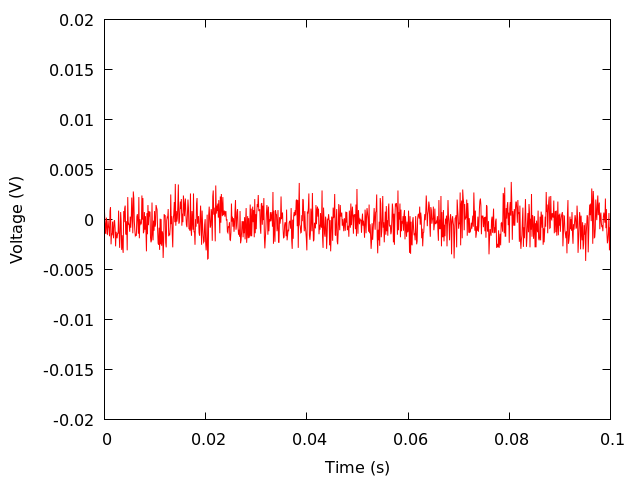
\includegraphics[width=\graphwidth]{./res/image/pos-noload-ripple.png}
    \caption{Measured no load positive rectifier ripple.}
    \label{fig:pos_noload_ripple}
\end{figure}

\newpage

\subsection{Negative Regulator}

\subsubsection{Simulated}

\begin{figure}[H]
    \centering
    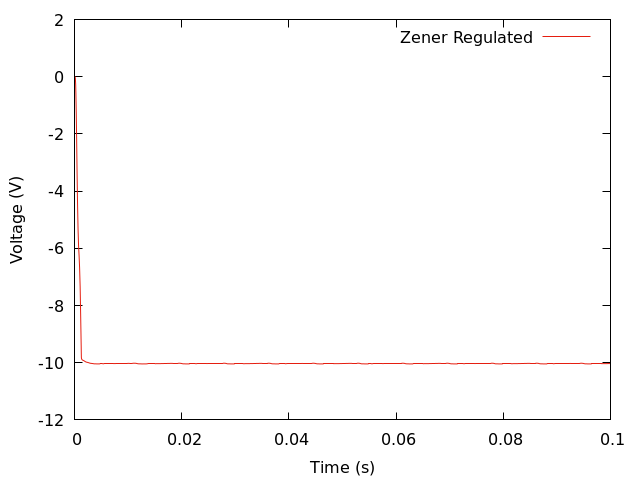
\includegraphics[width=\graphwidth]{./res/image/sim-neg-regulated-noload.png}
    \caption{Simulated zener no load regulation.}
    \label{sim:neg_noload}
\end{figure}


\begin{figure}[H]
    \centering
    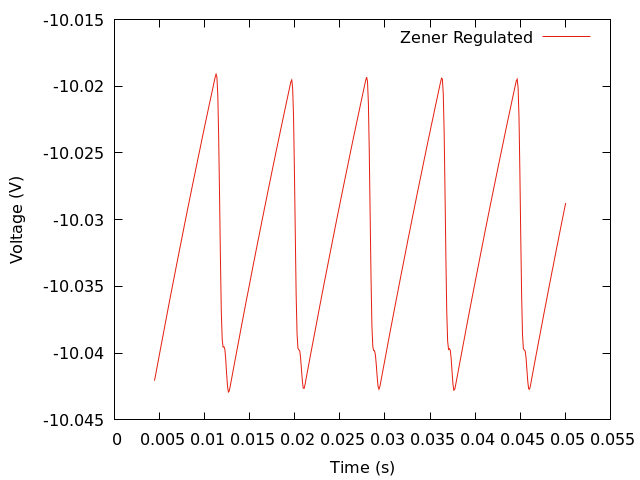
\includegraphics[width=\graphwidth]{./res/image/sim-neg-regulated-noload-ripple.png}
    \caption{Simulated zener no load ripple.}
    \label{sim:neg_noload_ripple}
\end{figure}

\begin{figure}[H]
    \centering
    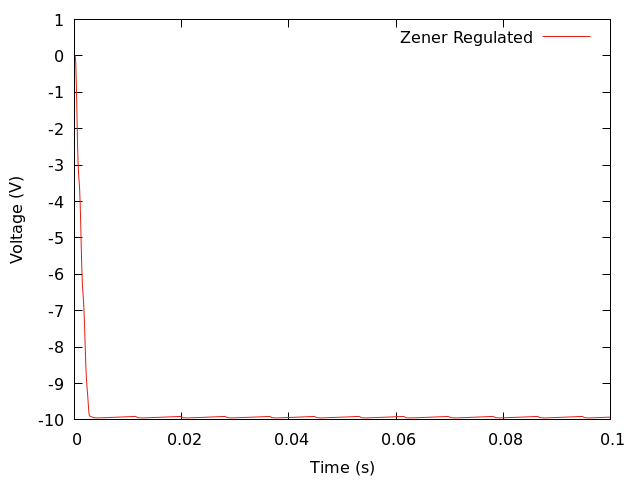
\includegraphics[width=\graphwidth]{./res/image/sim-neg-regulated-load.png}
    \caption{Simulated zener full load regulation.}
    \label{sim:neg_load}
\end{figure}

\begin{figure}[H]
    \centering
    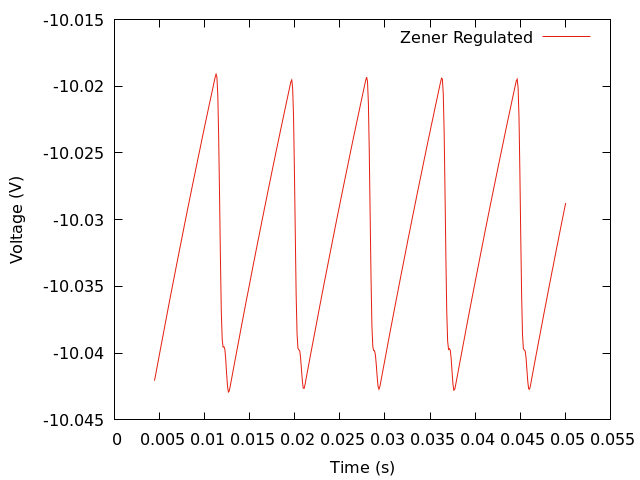
\includegraphics[width=\graphwidth]{./res/image/sim-neg-regulated-noload-ripple.png}
    \caption{Simulated zener full load ripple.}
    \label{neg:neg_noload_ripple}
\end{figure}

\subsubsection{Measured}

\begin{figure}[H]
    \centering
    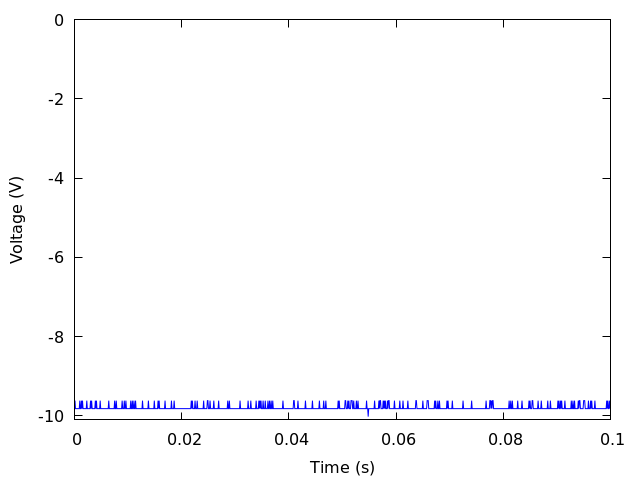
\includegraphics[width=\graphwidth]{./res/image/neg-full-load.png}
    \caption{Measured zener full load regulation.}
    \label{fig:neg_load_}
\end{figure}

\begin{figure}[H]
    \centering
    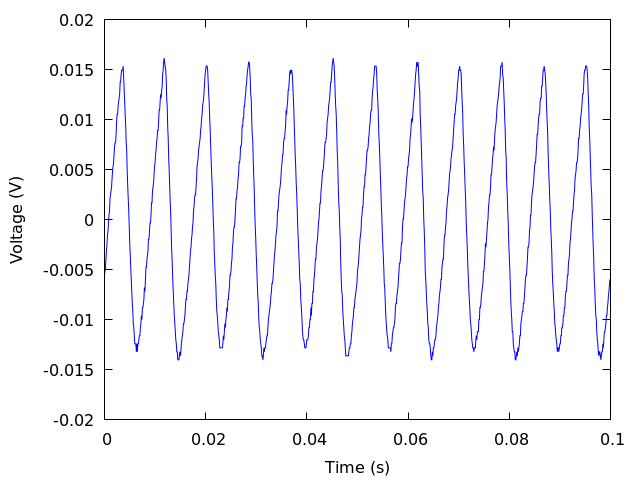
\includegraphics[width=\graphwidth]{./res/image/neg-full-load-ripple.png}
    \caption{Measured zener full load ripple.}
    \label{fig:neg_load_ripple}
\end{figure}

\end{appendix}


\end{document}
